\begin{frame}{Related work}
	\begin{itemize}
		\item \emph{Redirected Walking in Virtual Environments} by James Walker \note{Our experiment is a reproduction study of this}
		\item \emph{Analyses of human sensitivity to redirected walking} by F. Steinicke et al.
		\item \emph{Estimation of detection thresholds for redirected walking techniques} by F. Steinicke et al.
	\end{itemize}
\end{frame}

\begin{frame}{Redirected Walking in Virtual Environments}
	\only<1>{\begin{figure}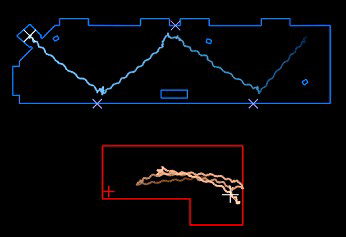
\includegraphics[height=0.8\textheight]{walker-1}\end{figure}\note{This figure shows a small scale example of exploring a larger virtual world in a smaller physical space}}
	\only<2>{\begin{figure}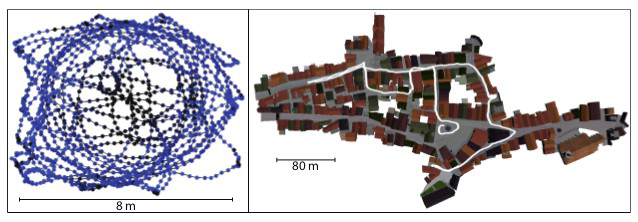
\includegraphics[width=\textwidth]{walker-3}\end{figure}\note{Now, this next figure is a bit more interesting. As you can see, with very limited physical space, people are able to explore a virtual world that is almost two magnitudes bigger.}}
\end{frame}

\begin{frame}{Analyses of human sensitivity to redirected walking}
	\begin{figure}
		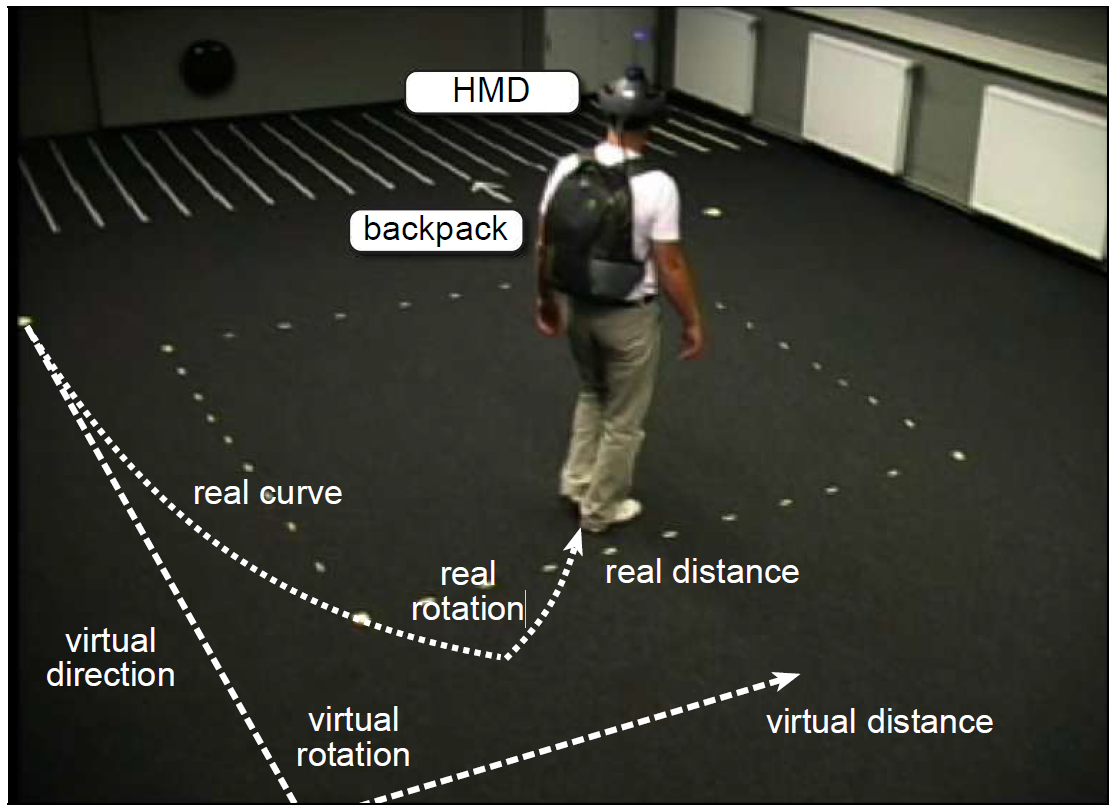
\includegraphics[height=0.8\textheight]{steinicke-1}
	\end{figure}
	\note{So this study laid the groundwork for the work of Walker. As you can see here this is the experimental setup they used.}
\end{frame}
